\documentclass{article}
\usepackage[margin=1in]{geometry}
\usepackage{amsmath,amsthm,amssymb}
\usepackage{bbm,enumerate,mathtools}
\usepackage{tikz,pgfplots}
\usepackage{chessboard}
\usepackage[hidelinks]{hyperref}
\usepackage{multicol} % Problem 35

\newenvironment{question}{\begin{trivlist}\item[\textbf{Question.}]}{\end{trivlist}}
\newenvironment{note}{\begin{trivlist}\item[\textbf{Note.}]}{\end{trivlist}}
\newenvironment{references}{\begin{trivlist}\item[\textbf{References.}]}{\end{trivlist}}
\newenvironment{related}{\begin{trivlist}\item[\textbf{Related.}]\end{trivlist}\begin{enumerate}}{\end{enumerate}}


\begin{document}
Consider all rectangles with all corners on gridpoints on an $n \times m$ grid.
\begin{figure}[!h]
  \centering
  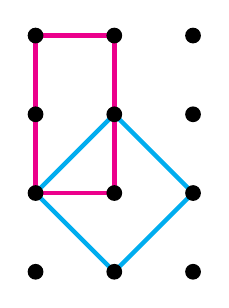
\begin{tikzpicture}
    \draw[magenta, ultra thick] (1,4)--(2,4)--(2,2)--(1,2)--(1,4);
    \draw[cyan, ultra thick]  (1,2)--(2,3)--(3,2)--(2,1)--(1,2);

    \foreach \x in {1,...,3} {
      \foreach \y in {1,...,4} { \fill (\x,\y) circle (0.1cm); }
    }
  \end{tikzpicture}
  \caption{
    An example of two rectangles with all corners on gridpoints of a
    $3 \times 4$ grid.
  }
\end{figure}

\begin{question}
  How many such rectangles exist?
\end{question}
\begin{related}
  \item How many squares exist? Rhombuses? Parallelograms? Kites? Quadrilaterals?
  \item How many right triangles?
  \item What if this is done on an $n \times m \times k$ grid?
  \item What if the rectangles must be diagonal?
  \item What if this is done on a triangular lattice?
  \item How many tetrahedra are in an $n$-sided tetrahedra?
\end{related}
\begin{references}
  \item See problem 1.
\end{references}
\end{document}
